\documentclass[11pt,letterpaper]{article}
\usepackage[letterpaper,margin=0.75in]{geometry}
\usepackage[T1]{fontenc}
\usepackage{lmodern}
\usepackage{microtype}
\usepackage{enumitem}
\usepackage{booktabs}
\usepackage{amsmath}
\usepackage{graphicx}
\usepackage[hidelinks]{hyperref}
\urlstyle{same}
\renewcommand{\UrlFont}{\itshape}
\setlist{nosep,leftmargin=*}
\renewcommand{\labelitemi}{$\bullet$}
\setlength{\parskip}{3pt}
\setlength{\parindent}{0pt}
\usepackage{titlesec}
\titlespacing*{\section}{0pt}{7pt}{2pt}
\titlespacing*{\subsection}{0pt}{5pt}{1pt}
\titleformat{\section}{\normalsize\bfseries}{\thesection.}{0.4em}{}
\titleformat{\subsection}{\normalsize\bfseries}{\thesubsection}{0.4em}{}
\setlength{\emergencystretch}{3em}
\setlength{\textfloatsep}{8pt}
\setlength{\floatsep}{6pt}
\setlength{\abovecaptionskip}{3pt}
\usepackage[font=small]{caption}

\begin{document}

\begin{center}
{\large\bfseries Content Effects in LLM Syllogistic Reasoning:\\ The Right Prompting Fix Depends on the Model (SemEval-2026 Task 11)}\\[3pt]
Meghana Nataraju \quad University of Illinois Chicago \quad CS 421 
\end{center}

\section{Task and Setup}
\textbf{Task.} SemEval-2026 Task 11 asks whether a syllogism is \emph{logically valid}, that is, whether its conclusion must follow from its premises, independently of whether the conclusion is believable (its \emph{plausibility}) \cite{valentino}. Language models, like humans, tend to accept believable conclusions and reject unbelievable ones regardless of logic: the \emph{content effect} \cite{dasgupta}. Subtask~1 gives English syllogisms with two premises; Subtask~2 adds irrelevant premises and also asks which premises are needed. Subtasks~3 and~4 repeat these in 11 other languages. I address Subtasks~1 and~2, asking: how large is the content effect in small open LLMs, which low-cost prompting methods reduce it, and do irrelevant premises make it worse?

\textbf{Official metric.} Let accuracy (\%) be computed separately in four groups: valid--plausible ($a_{VP}$), valid--implausible ($a_{VI}$), invalid--plausible ($a_{IP}$), invalid--implausible ($a_{II}$). The \emph{intra} content effect is $(|a_{VP}-a_{VI}| + |a_{IP}-a_{II}|)/2$ (does plausibility change accuracy for a fixed validity label?); the \emph{cross} content effect is $(|a_{VP}-a_{IP}| + |a_{VI}-a_{II}|)/2$ (does validity change accuracy for a fixed plausibility?). The total content effect TCE is their mean (0 = unbiased; lower is better). The ranking score is CS $= \mathrm{Acc} / (1 + \ln(1 + \mathrm{TCE}))$ with Acc the overall validity accuracy (\%). For Subtask~2, Acc is replaced by $(\mathrm{Acc} + F_1)/2$, where $F_1$ is premise-selection F1 computed only over gold-valid items: per item, precision and recall of the predicted premise set against the gold set; these are averaged over items, and $F_1 = 2PR/(P+R)$ of the two averages (\%). The log penalty is steep: a TCE of only 1.6 halves CS. I call the official scoring functions directly; predicting ``valid'' for every Subtask~1 test item gives Acc 50.26, TCE 50.0, CS 10.19, confirming the setup.

\textbf{Changes since the proposal.} (1) QLoRA fine-tuning and the planned solver-based upper bound were dropped for time; the leaderboard's solver systems (CS 100) serve as the reference instead. (2) Prompts were written once and not tuned on the dev set, so dev and test were run together after the fact. (3) Because decoding is greedy, repeated runs are identical, so the planned multiple seeds were replaced by bootstrap confidence intervals. (4) Subtask~2 uses the two 8B models only. Subtask~3 was dropped, as planned.

\section{Data}
I used the official public repository (commit \textit{6f71ea8}) \cite{repo}: 960 English training syllogisms (234--246 per validity--plausibility group), the Subtask~1 test set and the Subtask~2 test set, all with gold labels. From training, I removed 2 items whose text also appears in the test set and held out a balanced dev set of 160 items (40 per group, seed 42); the remaining 798 items were not needed because no model was trained. Subtask~1 syllogisms average 25 words. Subtask~2 items have 5 to 7 premises (2 relevant plus 3 to 5 distractors; 54 words on average); every valid item lists exactly 2 relevant premises. There is no Subtask~2 training or dev data, so Subtask~2 prompts were reused unchanged.

\textbf{Differences from the published data.} The overview paper reports 192 test items per subtask; the public files contain 191 (Subtask~1) and 190 (Subtask~2). In Subtask~1 one invalid--plausible item is missing (47 instead of 48 per group); Subtask~2's groups are 48/47/45/50 (VP/VI/IP/II). The repository does not document why items are missing; the most likely cause is items removed from the public release. Each missing item can move overall accuracy by about 0.5 points and a group accuracy by about 2 points, so leaderboard comparisons are approximate.

\section{Approach}
\textbf{Models and libraries.} Three instruction-tuned models from Hugging Face: Llama~3.2 3B Instruct, Llama~3.1 8B Instruct and Qwen3 8B (thinking mode off). All run in 4-bit NF4 quantization with float16 compute (\textit{transformers}, \textit{bitsandbytes}, \textit{accelerate}, PyTorch) on one free Google Colab T4 (16\,GB). No external data and no fine-tuning were used.

\textbf{Reading the answer.} Rather than generating text and parsing it, each prompt asks ``Is the argument logically valid? Answer with Yes or No only.'' and I run a single forward pass. From the next-token distribution I take the log-probabilities of the first token of ``Yes''/``yes'' and ``No''/``no'' (summed over variants with log-sum-exp), and $P(\text{Yes}) = \sigma(\log p_\text{Yes} - \log p_\text{No})$; valid if $P(\text{Yes}) \ge 0.5$. I expected this to work because instruction-tuned models are trained to answer yes/no questions with exactly these tokens; it also never fails to parse and gives a confidence score. Prompts use each model's chat template; batches are left-padded so the last position is the real last token, and only the last position's scores are computed (\textit{logits\_to\_keep=1}) to save memory.

\textbf{Three methods.}
\begin{itemize}
  \item \textbf{Zero-shot}: ``Decide whether the following argument is logically valid. An argument is valid if the conclusion must follow from the premises, whether or not the premises or conclusion are true in the real world.'' followed by the argument and the Yes/No question.
  \item \textbf{Chain-of-thought (CoT)}: the same definition, then ``Think step by step about the logical structure only, ignoring whether the statements are true in reality. Keep your reasoning short.'' The model generates up to 256 tokens (384 for Subtask~2) greedily; I then append ``Final answer (Yes or No):'' and read $P(\text{Yes})$ as above. Expected benefit: explicit steps should focus the model on form.
  \item \textbf{Abstraction}: the model first rewrites the argument, replacing each term with a capital letter (A, B, C), using the same letter for the same term (up to 128 tokens; 256 for Subtask~2). A zero-shot judge then sees \emph{only} the rewrite. Expected benefit: ``All A are B'' carries no believability, so the cue behind the content effect is removed.
\end{itemize}
\textbf{Premise selection (Subtask~2).} The argument is split into sentences at ``.'', ``!'' or ``?''; the last sentence is the conclusion. Premises are shown numbered, with ``Which premises are needed to logically derive the conclusion? Usually exactly two are needed. Answer with the numbers \dots''. The model's reply is pre-filled with ``Needed premises:'' and it generates 12 tokens; numbers on the first line are mapped from 1-based to 0-based. Without the pre-fill, Qwen3 explained first and was cut off (F1 0.0); with it, F1 rose to 84.6, and Llama's from 81.6 to 92.1. Premises are output for every item; the official F1 ignores gold-invalid items.

\textbf{Statistics.} 95\% bootstrap intervals use 2000 resamples of test items; method comparisons use paired bootstrap tests on the same resampled items (two-sided). Code: \url{https://github.com/MeghanaNatraj/syllogism-content-effect}.

\section{Results}

\begin{table}[t]
\centering\small
\begin{tabular}{@{}llccc@{}}
\toprule
Model & Method & Accuracy & TCE $\downarrow$ & CS \\
\midrule
Llama 3.2 3B & Zero-shot & 59.7 {\scriptsize[52.9, 66.5]} & 53.8 {\scriptsize[42.3, 65.2]} & 11.93 \\
 & CoT & 62.3 {\scriptsize[55.5, 69.1]} & 34.1 {\scriptsize[27.2, 40.8]} & 13.67 \\
 & Abstraction & 60.7 {\scriptsize[53.9, 67.5]} & 17.5 {\scriptsize[13.2, 27.4]} & 15.50 \\
\addlinespace[2pt]
Llama 3.1 8B & Zero-shot & 67.0 {\scriptsize[60.2, 73.8]} & 41.3 {\scriptsize[29.6, 52.5]} & 14.12 \\
 & CoT & 71.7 {\scriptsize[64.9, 78.0]} & 27.4 {\scriptsize[17.5, 39.2]} & 16.50 \\
 & Abstraction & 70.7 {\scriptsize[63.9, 77.0]} & \textbf{8.3} {\scriptsize[4.5, 19.2]} & 21.86 \\
\addlinespace[2pt]
Qwen3 8B & Zero-shot & 66.5 {\scriptsize[59.7, 73.3]} & 23.3 {\scriptsize[15.3, 36.1]} & 15.87 \\
 & CoT & \textbf{84.3} {\scriptsize[78.5, 89.0]} & \textbf{6.3} {\scriptsize[3.0, 14.6]} & \textbf{28.28} \\
 & Abstraction & 68.6 {\scriptsize[61.8, 74.9]} & 24.0 {\scriptsize[16.9, 31.5]} & 16.26 \\
\midrule
\multicolumn{2}{@{}l}{Always ``valid'' (trivial)} & 50.3 & 50.0 & 10.19 \\
\multicolumn{2}{@{}l}{Published zero-shot baselines \cite{valentino}} & 56.5--97.4 & 4.2--49.2 & 11.87--36.62 \\
\multicolumn{2}{@{}l}{Top shared-task systems (10 teams)} & 100 & 0 & 100 \\
\bottomrule
\end{tabular}
\caption{Subtask~1 test results (191 items) with 95\% bootstrap intervals. Published baselines are participant-reported zero-shot open models in the overview paper's Table~2 (e.g., Llama~3.1 8B Instruct: Acc 58.33, TCE 49.15, CS 11.87; Llama~3.2 3B Instruct: 57.64, 29.81, 13.02).}
\label{tab:st1}
\end{table}

\begin{figure}[t]
\centering
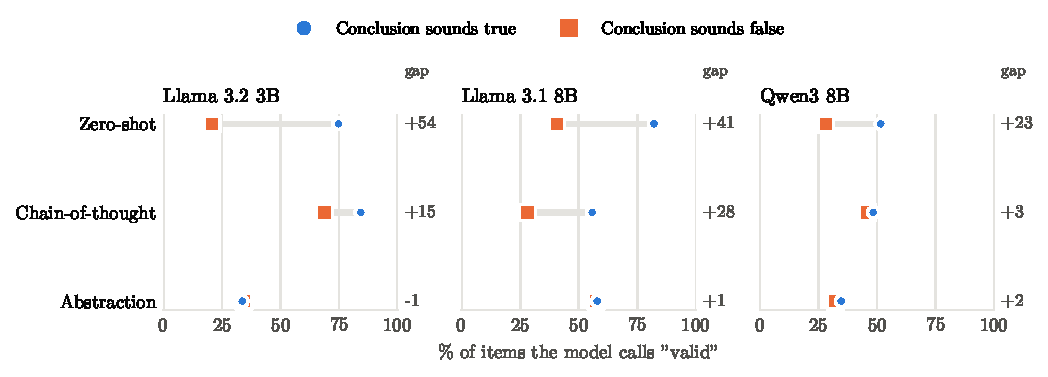
\includegraphics[width=\linewidth]{fig1_says_valid_gap.pdf}
\caption{Share of Subtask~1 test items labeled ``valid'', by whether the conclusion sounds true (circle) or false (square). The gap is the content effect: abstraction closes it for both Llama models, CoT for Qwen3.}
\label{fig:gap}
\end{figure}

\textbf{Subtask~1} (Table~\ref{tab:st1}, Figure~\ref{fig:gap}). Every zero-shot model shows a strong content effect: Llama~3.2 3B calls 75\% of believable conclusions valid but only 21\% of unbelievable ones. The methods help different models (Table~\ref{tab:paired}). Abstraction cuts TCE by 36 and 33 points for the two Llama models ($p<0.001$) but does nothing for Qwen3. CoT lowers TCE for all three models, yet only Qwen3 also becomes more accurate (+17.8 points, $p<0.001$), giving the best system: Qwen3 8B + CoT, CS 28.28. No method significantly changes either Llama model's accuracy: the gains are in bias, not correctness. The 160-item dev set shows the same pattern (Llama abstraction: TCE $-$32.5 and $-$31.3; Qwen3 CoT: accuracy +16.9).

\textbf{In context.} All our systems beat the trivial baseline and fall inside the published zero-shot range (CS 11.87--36.62), far below the top score of 100. Among the 34 entries reported in the overview paper's results table (mean CS 58.1, median 44.5, by my count), CS 28.28 would rank about 30th. All entries scoring 100 translate the argument into logic and check it with a symbolic solver; ours are end-to-end LLMs. Our zero-shot Llama~3.1 8B is more accurate than the published number (67.0 vs.\ 58.3) at a similar TCE, while our Llama~3.2 3B has a much larger TCE (53.8 vs.\ 29.8): the prompt wording clearly matters.

\textbf{Comparability.} Our scores use the public gold labels with the official functions, not the shared-task submission server, on 191 and 190 instead of 192 items (Section~2). Prompts were fixed before the test run, and no test labels were used to choose anything. Comparisons with the leaderboard are therefore close but not exact.

\begin{table}[t]
\centering\small
\begin{tabular}{@{}llcc@{}}
\toprule
Model & Method vs.\ zero-shot & $\Delta$ Accuracy & $\Delta$ TCE \\
\midrule
Llama 3.2 3B & CoT & +2.6 ($p=0.57$) & $-$19.6 ($p=0.004$) \\
 & Abstraction & +1.0 ($p=0.88$) & $-$36.3 ($p<0.001$) \\
Llama 3.1 8B & CoT & +4.7 ($p=0.23$) & $-$13.9 ($p=0.039$) \\
 & Abstraction & +3.7 ($p=0.36$) & $-$33.0 ($p<0.001$) \\
Qwen3 8B & CoT & +17.8 ($p<0.001$) & $-$17.1 ($p=0.002$) \\
 & Abstraction & +2.1 ($p=0.60$) & +0.6 ($p=1.0$) \\
\bottomrule
\end{tabular}
\caption{Paired bootstrap tests against zero-shot, Subtask~1 test set.}
\label{tab:paired}
\end{table}

\begin{table}[t]
\centering\small
\begin{tabular}{@{}llccccc@{}}
\toprule
 & & \multicolumn{2}{c}{Accuracy} & \multicolumn{2}{c}{TCE $\downarrow$} & \\
\cmidrule(lr){3-4}\cmidrule(lr){5-6}
Model & Method & ST1 & ST2 & ST1 & ST2 & ST2 CS \\
\midrule
Llama 3.1 8B & Zero-shot & 67.0 & 61.1 & 41.3 & 57.6$^{*}$ & 15.10 \\
 & CoT & 71.7 & 61.6$^{*}$ & 27.4 & 19.7 & 19.06 \\
 & Abstraction & 70.7 & 61.1$^{*}$ & 8.3 & \textbf{3.5} & \textbf{30.58} \\
\addlinespace[2pt]
Qwen3 8B & Zero-shot & 66.5 & 74.7 & 23.3 & 11.0 & 22.83 \\
 & CoT & 84.3 & \textbf{84.2} & 6.3 & 11.5 & 23.91 \\
 & Abstraction & 68.6 & 63.7 & 24.0 & 34.2$^{*}$ & 16.25 \\
\bottomrule
\end{tabular}
\caption{Without (ST1) and with (ST2) irrelevant premises, test sets. $^{*}$: the 95\% bootstrap interval of the change excludes zero. Premise F1: 92.1 (Llama), 84.6 (Qwen3). Trivial baseline (always valid, no premises): CS 5.07; top systems: 100.}
\label{tab:st2}
\end{table}

\begin{figure}[t]
\centering
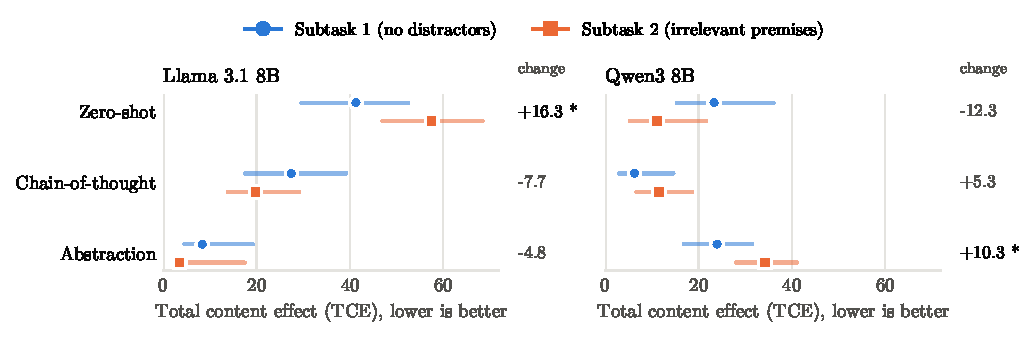
\includegraphics[width=\linewidth]{fig2_distractor_tce.pdf}
\caption{TCE without and with irrelevant premises, 95\% bootstrap intervals. Starred changes exclude zero.}
\label{fig:distractor}
\end{figure}

\textbf{Subtask~2} (Table~\ref{tab:st2}, Figure~\ref{fig:distractor}). Irrelevant premises significantly increased the content effect in two of six settings: Llama zero-shot (+16.3) and Qwen3 abstraction (+10.3). They cost Llama about 10 accuracy points with CoT and abstraction, while Qwen3 + CoT kept 84\%. Llama + abstraction remains nearly unbiased (TCE 3.5) and is the best Subtask~2 system (CS 30.58, about 9th of 12 reported entries; mean 49.8, top 100). So distractors do not uniformly increase bias; whether they do depends on the model and method. Since Subtask~1 and~2 contain different syllogisms, these are independent-sample comparisons.

\section{Analysis}

\textbf{Success: abstraction removes the cue.} ``\emph{There are some Ferraries that are things with wheels. Everything that is a Ferrari is a car. It follows that every car has wheels.}'' is invalid but believable. Llama~3.1 8B zero-shot calls it valid ($P(\text{Yes})=0.64$). Its rewrite, ``\emph{There are some A that are B. Everything that is an A is a C. It follows that every C is a B.}'', is judged invalid ($0.34$): with the true-sounding words gone, the model sees the form. Figure~\ref{fig:gap} shows this at scale: for both Llama models the gap between believable and unbelievable conclusions shrinks from 41--54 points to about 1.

\textbf{Failure: the rewrite itself is wrong.} ``\emph{Every single object can fly. It is known that some boats cannot fly. It follows that some boats are not objects.}'' is valid but absurd. Llama~3.1 8B rewrote it as ``\emph{A. Every single X can fly. It is known that some Y cannot fly. It follows that some Y are not Z.}'': ``objects'' received two letters (X and Z), breaking the link between premise and conclusion, so the judge correctly found the \emph{rewrite} invalid. Since a Subtask~1 syllogism has exactly three terms, I counted rewrites using exactly three letters (a heuristic). Only 44.0\% of Llama~3.1 8B's rewrites were clean (Llama~3.2 3B: 77.0\%, Qwen3: 83.8\%), and its accuracy is 77.4\% on clean rewrites vs.\ 65.4\% otherwise. Abstraction quality, not the idea itself, limits it. With Subtask~2's longer arguments there are more terms to map, matching the drop in Qwen3's abstraction accuracy.

\textbf{Why abstraction does nothing for Qwen3.} Qwen3 rewrites cleanly, but its judge leans toward ``invalid'' on abstract forms (it says valid to only 34\% of items). Most of its remaining TCE is the intra-plausibility part (33.1 on test): within each plausibility group, valid and invalid arguments get very different accuracy, which reflects a general lean towards ``invalid''. The cross-plausibility part, the actual plausibility effect, is smaller (14.8 on test, 2.5 on dev). The metric folds both into one number, so a method can reduce the plausibility effect without lowering TCE.

\textbf{Failure: CoT invents premises.} For the same flying-objects item, Llama~3.1 8B's reasoning said the argument ``is based on the assumption that `object' and `can fly' are equivalent'' and answered invalid. It added a requirement that is not part of the logic instead of applying the rule. Explicit appeals to real-world truth (``in reality'', ``real world'') appear in under 4\% of CoT texts, so the bias acts implicitly rather than through stated beliefs. For Qwen3, CoT is the most effective method, consistent with its training for step-by-step reasoning; Llama~3.2 3B with CoT instead calls 76\% of items valid, shifting its bias rather than removing it. Valid arguments with absurd conclusions are the hardest items for every method.

\section{Ethics and Limitations}
\textbf{Ethics.} The content effect matters beyond puzzles: a model that judges arguments by how believable their conclusions sound can be persuaded by fluent but invalid reasoning and can dismiss sound reasoning with surprising conclusions, which is risky when LLMs are used to check arguments in medical, legal or educational settings. The Subtask~2 result connects to prompt injection: irrelevant text increased an unprotected model's bias by 16 points. The plausibility labels encode one view of common sense in English (e.g., what counts as ``believable'' about animals, vehicles or food), so a system tuned to this data may not transfer to other languages or cultural assumptions, which is why the task's multilingual subtasks exist. A validity checker should never be presented as judging whether a conclusion is \emph{true}: a valid argument with false premises still has a false conclusion.

\textbf{Limitations.} I would not claim that any method is generally best: the effect depends on the model. Test sets have only about 190 items, so differences under roughly 10 TCE points are often not significant. Prompts were not tuned, Qwen3 was run with thinking mode off only, the abstraction and CoT checks are keyword heuristics, and Subtask~1 and~2 use different items. With another month I would (1) make abstraction reliable with a structured output that maps each term to one letter, then check validity with a small rule-based solver, the approach of the top systems; (2) test several prompt wordings on dev; (3) run Qwen3 with thinking on; (4) fine-tune with LoRA on the 798 training items with plausibility-flipping augmentation; and (5) extend to the multilingual subtasks.

\section{Conclusion}
This project investigated content effects in small open-weight language models through SemEval-2026 Task 11. The results demonstrate that prompting-based mitigation is model-dependent: abstraction substantially reduces content effects in Llama models, whereas chain-of-thought reasoning is more effective for Qwen3. Evaluation on Subtask 2 further shows that performance differences associated with distracting premises vary across model-method configurations. Although the proposed methods do not match the strongest neuro-symbolic systems, they demonstrate that computationally inexpensive prompting strategies can meaningfully improve reasoning robustness without fine-tuning. These findings highlight the importance of model-specific evaluation when designing content-independent reasoning systems.

\subsection*{Use of Generative AI}
I used an AI assistant (Claude) initially to help me understand the task, explore suitable approaches, and organize the project into a six-week plan with weekly objectives, tasks, and deliverables. It provided coding assistance while implementing data splitting and scoring and helped troubleshoot technical issues, including GPU memory limitations, package version incompatibilities, and premise-selection formatting problems. It also assisted in drafting the report based on my experimental results and generating the LaTeX code to structure and format my content appropriately.

\small
\begin{thebibliography}{9}\setlength{\itemsep}{1pt}
\bibitem{dasgupta} I.~Dasgupta, A.~K. Lampinen, S.~C.~Y. Chan, A.~Creswell, D.~Kumaran, J.~L. McClelland, and F.~Hill. 2022. Language models show human-like content effects on reasoning. \textit{arXiv:2207.07051}.
\bibitem{repo} Official SemEval-2026 Task 11 repository. \url{https://github.com/neuro-symbolic-ai/semeval_2026_task_11}
\bibitem{valentino} M.~Valentino, L.~Ranaldi, G.~Pucci, F.~Ranaldi, and A.~Freitas. 2026. SemEval-2026 Task 11: Disentangling content and formal reasoning in large language models. In \textit{Proceedings of the 20th International Workshop on Semantic Evaluation (SemEval-2026)}, pages 3716--3730. \url{https://aclanthology.org/2026.semeval-1.450/}
\end{thebibliography}

\end{document}
